% diagrams/english/muneco-nieve.tex -- el muñeco de nieve del jardín,
% para "Read and colour": el sombrero, la bufanda, la nariz de
% zanahoria, los ojos, los botones y los brazos de rama.
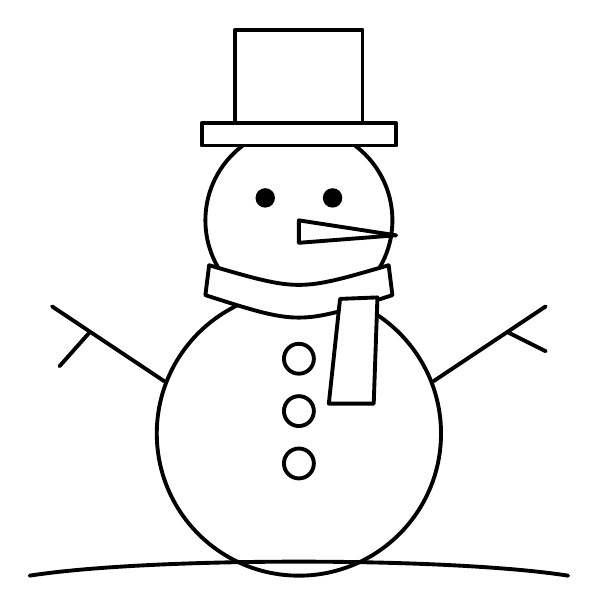
\begin{tikzpicture}[line width=1.4pt, line cap=round, line join=round, scale=0.95]
  % las dos bolas
  \filldraw[fill=white] (0,1.9) circle (1.9);
  \filldraw[fill=white] (0,4.75) circle (1.25);
  % los brazos de rama
  \draw (-1.8,2.6) -- (-3.3,3.6); \draw (-2.8,3.25) -- (-3.2,2.8);
  \draw (1.8,2.6) -- (3.3,3.6); \draw (2.8,3.25) -- (3.3,3.0);
  % la bufanda
  \filldraw[fill=white] (-1.25,3.75) .. controls (0,3.35) .. (1.25,3.75)
    -- (1.2,4.15) .. controls (0,3.8) .. (-1.2,4.15) -- cycle;
  \filldraw[fill=white] (0.55,3.7) -- (0.4,2.3) -- (1.0,2.3) -- (1.05,3.72) -- cycle;
  % los botones
  \foreach \y in {2.9,2.2,1.5} { \filldraw[fill=white] (0,\y) circle (0.2); }
  % los ojos y la nariz
  \fill (-0.45,5.05) circle (0.13); \fill (0.45,5.05) circle (0.13);
  \filldraw[fill=white] (0,4.75) -- (1.3,4.55) -- (0,4.45) -- cycle;
  % el sombrero
  \filldraw[fill=white] (-1.3,5.75) rectangle (1.3,6.05);
  \filldraw[fill=white] (-0.85,6.05) rectangle (0.85,7.3);
  % el suelo nevado
  \draw (-3.6,0) .. controls (-2,0.25) and (2,0.25) .. (3.6,0);
\end{tikzpicture}
